%!TEX root = ../thesis.tex

\subsection{提案モデルの識別可能性}

本節では、前節で定義したDAGモデルの識別可能性を証明する。
提案モデルは、連続変数と離散変数とが混在することを許容するDAGモデルであるため、
その特殊形として、全てが連続変数であるモデルや全てが離散変数であるモデルを考えることも可能である。
全てが連続変数である場合は、Additive Noise Modelとなり、
モデルの識別可能条件が複数証明されている\cite{Shimizu2006-yu}
\cite{Hoyer2008-oo}
\cite{Peters2013-eb}
\cite{Peters2014-ro}
\cite{Park2020-ey}。
また、全てが離散変数である場合は、QVF-DAGモデル\cite{Park2017-hw}となり、
識別可能性が既に証明されている\cite{Park2017-hw}。
そこで以下では、観測変数集合に連続変数と離散変数の両方が含まれる場合に関する識別可能条件について議論する。
まず、証明の方針について直感的な理解を得るために、
図\ref{fig:prop_three_variate}のような3変数モデルを用いてその識別可能性を示す。
ここで$X,Z$は連続変数、$Y$は離散変数であるとする。
図\ref{fig:prop_three_variate}の3つの因果グラフから生成される分布は、
いずれも$X \indep Z | Y$という条件付き独立関係が成立しており、
因果マルコフ条件のみでは識別できない例である。
しかし、以下で示すように、提案モデルの特徴を利用すると識別することが可能である。

\begin{align*}
  G_1 \colon & X = \theta_{X} + e_X, \quad e_X \sim N(0, \sigma_X^2) \\
             & Y|X \sim \mathit{Poisson}(\lambda), \quad \log(\lambda) = \theta_Y + \theta_{YX}X \\
             & Z = \theta_Z + \theta_{ZY}Y + e_Z, \quad e_Z \sim N(0, \sigma_Z^2)
\end{align*}

\begin{align*}
  G_2 \colon & X = \theta_X + \theta_{XY}Y + e_X, \quad e_X \sim N(0, \sigma_X^2) \\
             & Y|Z \sim \mathit{Possion}(\lambda), \quad \log(\lambda) = \theta_Y + \theta_{YZ}Z \\
             & Z = \theta_{Z} + e_Z, \quad e_Z \sim N(0, \sigma_Z^2)
\end{align*}

\begin{align*}
  G_3 \colon & X = \theta_X + \theta_{XY}Y + e_X, \quad e_X \sim N(0, \sigma_X^2) \\
             & Y \sim \mathit{Poisson}(\lambda) \\
             & Z = \theta_{Z} + e_Z, \quad e_Z \sim N(0, \sigma_Z^2)
\end{align*}

\begin{figure}[ht]
  \centering
  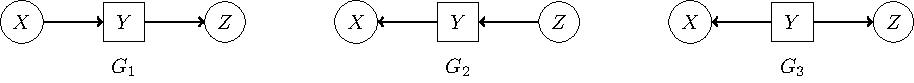
\includegraphics{./picture/prop_three_variate.pdf}
  \caption{3変数のDAGモデル}
  \label{fig:prop_three_variate}
\end{figure}

命題\ref{prop:MRS}より、$G_1, G_2$においては
\begin{align*}
  E(Y^2) > E(Y) + E(Y)^2
\end{align*}
である一方で、$G_3$においては
\begin{align*}
  E(Y^2) = E(Y) + E(Y)^2
\end{align*}
となる。
よって、離散変数のモーメント比~\eqref{eq:MRS}が1か1以上かを確かめることで
$G_1, G_2$と$G_3$は識別可能である。

次に$G_1$について、もし連続変数$X, Z$の誤差変数の分散が
$\sigma_X^2 < \sigma_Z^2 + \mathit{Var}(E(Z|Y))$を満たすならば、
全分散の公式を用いて以下が成り立つ。
\begin{align*}
  \mathit{Var}(Z) &= E(\mathit{Var}(Z|Y)) + \mathit{Var}(E(Z|Y)) \\
                  &= \sigma_Z^2 + \mathit{Var}(E(Z|Y)) \\
                  &> \sigma_X^2 \\
                  &= \mathit{Var}(X)
\end{align*}

よって、$X$のほうが因果順序が早いことが分かる。
つまり、誤差変数の分散が$\sigma_X^2 < \sigma_Z^2 + \mathit{Var}(E(Z|Y))$を満たすならば、
$G_1$の因果順序を特定することが可能である。

$G_2$についても同様に、
連続変数$X, Z$の誤差変数の分散が、
$\sigma_Z^2 < \sigma_X^2 + \mathit{Var}(E(X|Y))$を満たすならば、
真の因果順序$\pi = (Z, Y, X)$を特定することが可能である。


ここからは、上記の3変数モデルでの証明の方針を拡張し、
提案モデルが一般的な$p$変数の場合においても識別可能であることを証明する。

まず初めに、提案モデルにおける離散変数に関して、
命題\ref{prop:MRS}と同様の関係が成立していることを示す。

\begin{lemm}
  提案モデルにおいて、
  離散変数が割り当てあられた任意の頂点$j \in D$、任意の集合$S_j \subset Nd(j)$に関して、
  以下のモーメント関係が成立している。
  \begin{equation}
    \frac{E(X_j^2)}
    {E \left[ \beta_0 E(X_j | X_{S_j}) + (\beta_1 + 1)E(X_j | X_{S_j})^2 \right]}
    \geq 1
    \label{prop_MRS}
  \end{equation}
  等号成立は、$S_j$が頂点$j \in D$の親変数全てを含むとき($Pa(j) \subset S_j$)である。
  \label{lem_prop_MRS}
\end{lemm}

\begin{proof}
  提案モデルにおいて、離散変数が割り当てられた頂点は、式~\eqref{QVF_prop}を満たすため、
  任意の変数$X_j \in X_D$について以下の関係が成り立つ。
  \begin{equation*}
    E(X_j^2) = \beta_0 E(X_j) + (\beta_1 + 1)E(X_j)^2
  \end{equation*}

  ここで、記号の簡単の簡単のために、関数$f(\mu) = \beta \mu + (\beta_1 + 1) \mu^2$を定義する。
  すると、任意の頂点$j \in D$、任意の空でない集合$S_j \subset Nd(j)$について、以下のように書ける。
  \begin{equation}
    \begin{split}
      E(X_j^2 | S_j) &= E(E(X_j^2 | X_{Pa(j)}) | S_j) \\
                     &= E(f(E(X_j | X_{Pa(j)})) | S_j)
    \end{split}
    \label{prop_moment}
  \end{equation}
  提案モデルにおいては連続変数と離散変数が混在するモデルを考えているため、
  離散変数が割り当てられた頂点$j \in D$の非子孫の集合$Nd(j)$には、
  連続変数と離散変数の両方が含まれている可能性がある。
  つまり、式~\eqref{prop_moment}は$S_j$に連続変数と離散変数のどちらが含まれていても成立する。

  以降の証明は、命題\ref{prop:MRS}の証明と同様である。

  \qed
\end{proof}

補題\ref{lem_prop_MRS}で証明したモーメント関係は$p$変数の提案モデルでも利用することができる。
つまり、式~\eqref{prop_MRS}が1に等しくなる$X_j \in X_D$が存在するかどうかを確認することによって、
因果順序の1番目の変数が離散変数か否かを判断することができ、
離散変数の場合はその変数を特定することができる。

\begin{theo}[提案モデルの識別可能性]
  \label{theo:prop_identifiability}
  定義\ref{prop_model}によって定義されるDAGモデルは、以下の仮定を満たすとき識別可能である。
  ここで、$\pi$はDAG $G$における因果順序を表す。
  \begin{enumerate}[label=(\Alph*)]
    \item
    連続変数が割り当てられた任意の頂点$j = \pi_m \in C, k \in De(j) \subset C$の
    データ生成過程における誤差変数の分散について、以下が満たされている。
    \begin{equation*}
      \sigma_j^2 < \sigma_k^2 + E(\mathit{Var}(E(X_k | X_{Pa(k)}) | X_{\pi_1}, \dots, X_{\pi_{m-1}}))
    \end{equation*}

    \item
    離散変数が割り当てあられた任意の頂点$j \in D$について、
    $\beta_{j1} > -1$が満たされている。
  \end{enumerate}
\end{theo}

仮定(B)は、ベルヌーイ分布や多項分布によるDAGモデルを除外するための仮定である。
なぜななら、ベルヌーイ分布や多項分布によるDAGモデルは識別不能であることが知られているためである\cite{Heckerman1995-es}。

以下では、定理\ref{theo:prop_identifiability}を証明する。

\begin{proof}
  一般性を失わずに、DAG $G$における因果順序が一意であり、$\pi = (\pi_1, \dots, \pi_p)$であると仮定する。
  また、簡単のために、$X_{1:j} = (X_{\pi_1}, X_{\pi_2}, \dots, X_{\pi_j})$、
  $X_{1:0} = \emptyset$と定義する。
  DAG $G$において、
  連続変数に割り当てられた変数からなる頂点の集合を$C$、
  離散変数に割り当てられた変数からなる頂点の集合を$D$とする。
  加えて、モーメント関連関数$f(\mu) = \beta_0 \mu + (\beta_1 + 1)\mu^2$を定義する。
  ここから数学的帰納法を用いて提案モデルの識別可能性を証明する。

  \begin{quote}
    \textbf{Step(1)}
    \begin{enumerate}[label=(\roman*)]
      \item
      \underline{$\pi_1 = j \in D$の場合} \\
      補題\ref{lem_prop_MRS}より、$E(X_{\pi_1}^2) = E(f(E(X_{\pi_1})))$が成立する。
      一方で、頂点$j \in D \backslash \{\pi_1\}$では、
      $E(X_j^2) > E(f(E(X_j)))$となる。
      そのため、因果順序が1番目の要素$\pi_1$は、
      $E(X_j^2) = E(f(E(X_j)))$となるような$j \in D$である。
      もし、そのような変数が存在しなければ、$X_{\pi_1}$は連続変数である。

      \item
      \underline{$\pi_1 = j \in C$の場合}\\
      定理\ref{theo:prop_identifiability}の仮定(A)より、
      任意の頂点$k \in C \backslash \{\pi_1\}$について、以下が成立する。
      \begin{align*}
        \mathit{Var}(X_{\pi_1}) &= \sigma_{\pi_1}^2 \\
                                &< \sigma_k^2 + \mathit{Var}(E(X_k | X_{Pa(k)})) \\
                                &= E(\mathit{Var}(X_k | X_{Pa(k)})) + \mathit{Var}(E(X_k | X_{Pa(k)})) \\
                                &= \mathit{Var}(X_k)
      \end{align*}
      よって、因果順序が1番目の要素$\pi_1$を特定することができる。
    \end{enumerate}
  \end{quote}

  \begin{quote}
    \textbf{Step(m-1)} \\
    因果順序が$(m-1)$番目の要素について、因果順序が早い$(m-1)$個の要素とその親が正しく推定されていると仮定する。
  \end{quote}

  \begin{quote}
    \textbf{Step(m)} \\
    因果順序が$m$番目の要素とその親について考える。
    \begin{enumerate}[label=(\roman*)]
      \item
      \underline{$\pi_m = j \in D$の場合} \\
      補題\ref{lem_prop_MRS}より、$E(X_{\pi_m}^2) = E(f(E(X_{\pi_m} | X_{1:(m-1)})))$が成立する。
      一方で、頂点$j \in \{\{ \pi_{m+1}, \dots, \pi_p\} \cap D\}$では、
      $E(X_j^2) > E(f(E(X_j | X_{1:(m-1)})))$となる。
      そのため、因果順序が$m$番目の要素$\pi_m$は、
      $E(X_j^2) = E(f(E(X_j | X_{1:(m-1)})))$となるような$j \in D$である。
      もし、そのような変数が存在しなければ、$X_{\pi_m}$は連続変数である。

      \item
      \underline{$\pi_m = j \in C$の場合} \\
      定理\ref{theo:prop_identifiability}の仮定(A)より、
      任意の頂点$k \in \{ \{ \pi_{m+1}, \dots, \pi_p \} \cap C \}$について、以下が成立する。
      \begin{align*}
        E(\mathit{Var}(X_{\pi_m} | X_{1:(m-1)}))
            &= \sigma_{\pi_m}^2 \\
            &< \sigma_k^2 + E(\mathit{Var}(E(X_k | X_{Pa(k)}) | X_{1:(m-1)})) \\
            &= E(E(\mathit{Var}(X_k | X_{Pa(k)}) | X_{1:(m-1)})) + E(\mathit{Var}(E(X_k | X_{Pa(k)}) | X_{1:(m-1)})) \\
            &= E(\mathit{Var}(X_k | X_{1:(m-1)}))
      \end{align*}
      よって、因果順序が$m$番目の要素$\pi_m$を特定することができる。

    \end{enumerate}
  \end{quote}


    各頂点の親に関しては、因果マルコフ条件に基づく
    $P(G)の因数分解$\eqref{eq:factorization}によって表現される
    条件付き独立関係と、
    因果極小性~\eqref{minimality}により導くことができる。
    つまり、以下を満たす頂点$k$を$\pi_m$の親として特定することができる。
    \begin{equation*}
      Pa(k) \colon = \{ k \in \{ \pi_1, \dots, \pi_{m-1} \} |
      X_k \notindep X_{\pi_m} | X_{\pi_1}, \dots, X_{\pi_{m-1}} \backslash X_k \}
    \end{equation*}

    よって、数学的帰納法により定理\ref{theo:prop_identifiability}の証明を完了する。

  \qed
\end{proof}
